% Chapter 1: Introduction

\chapter{Introduction}
\label{chap:introduction}

\section{Background and Motivation}
Large Language Models (LLMs) have emerged as the foundational substrate for contemporary natural language processing, powering applications spanning customer support, autonomous coding, personal productivity, and dialogue-driven interfaces. Commercial LLM providers (e.g., OpenAI, Anthropic, Google) operationalize inference billing on a per-token basis. Under this economic model, total operating expenditure is governed primarily by two factors:
\begin{enumerate}
    \item The total number of tokens ingested and generated per request.
    \item The operational capability tier of the underlying model (e.g., a compact 8B parameter model versus a frontier 120B+ parameter model).
\end{enumerate}

While prompt compression literature has demonstrated significant token reductions on clean monolingual English benchmarks \cite{jiang2023llmlingua, pan2024llmlingua2}, these techniques fail to account for the linguistic realities of multilingual populations in South Asia. In India, conversational discourse across messaging platforms, social media, and customer support frequently code-switches between Hindi and English (commonly termed \textit{Hinglish}), written predominantly in informal Romanized Latin script.

\section{The Tokenizer Tax and Linguistic Inequity}
Subword tokenizers, such as Byte-Pair Encoding (BPE) and WordPiece, are trained on corpora dominated by standard English text. When presented with code-mixed text or transliterated vernacular expressions, these tokenizers exhibit severe subword fragmentation \cite{petrov2023language}. 

\begin{figure}[htbp]
    \centering
    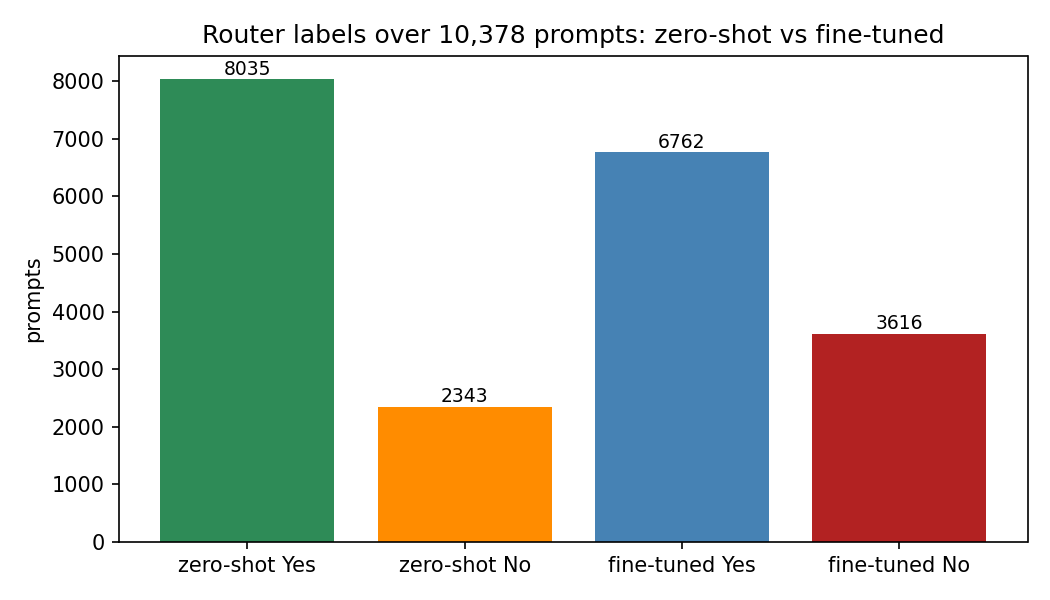
\includegraphics[width=0.85\linewidth]{Figures/fig_labels.png}
    \caption{Empirical label distribution shift across router training and complexity grading on code-mixed queries.}
    \label{fig:label_shift}
\end{figure}

For instance, consider a standard query:
\begin{itemize}
    \item \textbf{English:} \textit{``Please explain the difference between a process and a thread.''} (12 tokens in OpenAI \texttt{cl100k\_base}).
    \item \textbf{Hinglish (Romanized):} \textit{``Bhai process aur thread ke beech ka difference simple shabdon mein samjha do.''} (27 tokens in OpenAI \texttt{cl100k\_base}).
\end{itemize}

Despite conveying identical semantic intent, the Romanized Hinglish prompt incurs more than twice the token billing and processing latency. This phenomenon—the \textbf{Tokenizer Tax}—imposes an implicit, regressive economic penalty on multilingual communities. 

Furthermore, a second compounding penalty—the \textbf{Reasoning Tax}—manifests when reasoning-focused models (e.g., DeepSeek-R1 class) silently allocate substantial chains of internal ``thinking tokens'' to parse transliterated and unstandardized syntax before emitting downstream responses.

\section{Research Objectives and Formal Hypotheses}
This thesis investigates whether prompt compression and cascade routing can be jointly engineered to eliminate linguistic token disparity without sacrificing conversational task fidelity. We formally pre-register four primary Research Questions (RQs):

\begin{itemize}
    \item \textbf{RQ1 (Transferability):} At what achieved compression ratio does downstream task success degrade in Hindi-English code-mixed dialogue compared to uncompressed input?
    \item \textbf{RQ2 (Economics):} What empirical token reduction and financial cost savings are realized per provider tier under metered serving price schedules?
    \item \textbf{RQ3 (Failure Mechanism):} Are accuracy losses concentrated uniformly across discourse, or are they concentrated in named entities, digits, code snippets, or transliterated segments?
    \item \textbf{RQ4 (Span Recovery):} Can a deterministic protected-span masking mechanism recover 100\% entity survival at identical achieved compression ratios?
\end{itemize}

\section{Key Contributions}
The primary contributions of this thesis are as follows:
\begin{enumerate}
    \item \textbf{5-Stage CPU-Efficient Prompt Compressor:} We develop an extractive compression pipeline combining phonetic consonant-skeleton normalization (\texttt{hinglish\_phash}), heuristic filler stripping, regex-based protected-span safety gates, and a 25-feature Linear-Chain Conditional Random Field (CRF) tagger executing in $<10$\,ms on CPU.
    \item \textbf{Zero-Loss Entity Protection:} We demonstrate that raw neural token classifiers suffer from a 20--31\% entity mangling rate on code-mixed text. Our fail-closed masking and byte-for-byte reinjection mechanism restores entity recall to exactly 1.000 across 680 evaluated dialogue rows.
    \item \textbf{Conformal Cascade Routing:} We deploy a fine-tuned ModernBERT-large router coupled with Hoeffding Learn-Then-Test (LTT) risk bounds to provably control the risk ($\alpha \le 0.05$) of dispatching complex queries to compact open-source models (Groq Llama-3-8B) versus frontier models (GPT-4o).
    \item \textbf{12-Module OpenAI-Compatible Serving Gateway:} We integrate the compressor, router, evaluators, and transparency receipts into a production-grade FastAPI server supporting 20+ endpoints, streaming responses, and an open benchmark suite.
\end{enumerate}

\section{Thesis Organization}
The remainder of this thesis is structured as follows:
\begin{itemize}
    \item \textbf{Chapter \ref{chap:literature}} reviews foundational literature in prompt compression, multilingual tokenizer unfairness, cascade routing, and conformal risk control.
    \item \textbf{Chapter \ref{chap:methods}} details the mathematical formulation and software architecture of the 12-module gateway, the phonetic CRF compressor, and the conformal router.
    \item \textbf{Chapter \ref{chap:experiments}} presents the empirical evaluation on the PRESTO benchmark and Hinglish-Instruct dataset, providing ablation studies, cost analyses, and entity survival proofs.
    \item \textbf{Chapter \ref{chap:conclusion}} concludes the thesis with key findings, limitations, and future directions.
\end{itemize}
